\subsection{Analog-to-Digital Converter} \label{sec:ADC_teori}
Outputtet fra målinger foretaget på biologiske signaler fremstår som et analogt signal, der er kontinuert i tid og amplitude. For at kunne behandle signalet digitalt, skal signalet konverteres fra analog til digital, denne konverteringen sker ved anvendelse af en Analog-to-Digital Converter (ADC). Det analoge signal kvantificeres under konverteringen, hvilket gør, at det digitale signal bliver diskret i tid og amplitude \citep{webster1998}. Dette er illusteret på \autoref{fig:ADC_kon}. Konverteringsprocessen består af sampling og kvantificering \citep{morre2003}. 

\begin{figure}[H]
\centering
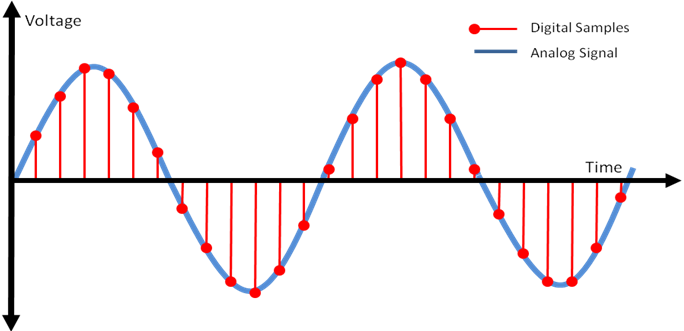
\includegraphics[width=0.7\textwidth]{figures/problemloesning/adc}
\caption{Illustration af konvertering fra analogt til digitalt signal. Den blå graf viser det analoge signal, mens den røde graf viser signalet efter det er konverteret til digitalt.}
\label{fig:ADC_kon}
\end{figure}

\noindent
Samplingsprocessen sker ved diskretisering i tidsdomænet, hvor det kontinuerte signal konverteres til et diskret signal. Det er vigtigt at vælge en passende samplingsfrekvens for at undgå, at information fra det oprindelige signal går tabt \citep{morre2003}. Ved for høj samplingsfrekvens vil en større mængde data opsamles og derved benytte mere plads og processering \citep{wolf2004}. En for lav samplingsfrekvens vil derimod kunne rekonstruere signalet, således kurven ikke kan repræsentere det oprindelige signal, hvilket fremgår som alias \citep{morre2003}. I følge Nyquists sætning er det hensigtsmæssigt, at samplingsfrekvensen er mindst det dobbelte af frekvensen i det oprindelige signal \citep{morre2003}. I praksis anbefales det dog at sample med det ti dobbelte.

Kvantificering sker ved diskretisering af amplituden. Det oprindelige signals amplitudeværdier inddeles ved kvantificering i trin. Værdierne mellem to trin repræsenteres af den samme digitale værdi. Dette gør at flere værdier kan ligge indenfor den samme digitale værdi \citep{morre2003}. Amplitudeniveauer, der er tilgængelige til at repræsentere det analoge signal, determineres af antal bits. Ved en højere bit værdi vil det analoge signal repræsenteres bedre, hvilket er illustreret på \autoref{fig:ADC_bit}.

\begin{figure}[H]
\centering
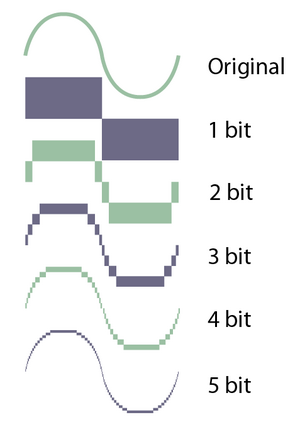
\includegraphics[width=0.5\textwidth]{figures/problemloesning/ADC_bit}
\caption{Illustration af betydningen af bits. Ved en større bitværdi vil signalet blive repræsenteres bedre.}
\label{fig:ADC_bit}
\end{figure}

En ADC med en opløsning på 12-bit inddeles i ${2}^{12}$, svarende til 4096 niveauer. Dette giver en repræsentation af værdier fra 0 til 4096 eller fra -2048 til 2047.  Den sensitivitet som ADC'ens sensitivitet kan opnå, omtales Least Significant Bit (LSB) og bestemmes ud fra \autoref{equ:LSB}, hvor Full Scale voltage Range (FSR) er det totale spændingsområde for ADC'en angivet i $V$, og $n$ er antallet af bits i ADC'en \citep{webster1998, wolf2004}.

\begin{equation} \label{equ:LSB}
LSB=\dfrac{FSR}{2^{n}}
\end{equation}

% = \dfrac{\dfrac{FSR}{{2}^{12}}}
\noindent
Hvis spændingen, der pålægges ADC'en overstiger dens arbejdsområde, vil dette resultere i, at signalet går i mætning \citep{webster1998, wolf2004}. 

\vspace{3mm}
\textbf{Krav:}
\begin{itemize}
%\item Skal have en samplingsfrekvens på $100~Hz$
\item Skal sample minimum tre inputs 
%\item Skal have en hastighed som ikke overskrider ADC'ens arbejdsområde \fxnote{Hvad vil hastigheden sige?}
\item Skal have en opløsning, der ikke forringer signalet.
\item Skal have en samplingsfrekvens omkring 10 gange større end den højeste signalfrekvens
\item Skal undgå, at signalet ikke overstiger ADC'ens arbejdsområde
%\item Skal have en opløsning på minimum 10 bit
%\item Skal modtage en spændingsforsyning på $XX~V$
%\item Skal have en tolerence på $XX~\%$ (kvatificeringsfejl?)
\end{itemize}

